% Created 2020-09-25 Fri 12:07
% Intended LaTeX compiler: pdflatex
\documentclass[presentation]{beamer}
\usepackage[utf8]{inputenc}
\usepackage[T1]{fontenc}
\usepackage{graphicx}
\usepackage{grffile}
\usepackage{longtable}
\usepackage{wrapfig}
\usepackage{rotating}
\usepackage[normalem]{ulem}
\usepackage{amsmath}
\usepackage{textcomp}
\usepackage{amssymb}
\usepackage{capt-of}
\usepackage{hyperref}
\usetheme{UoB}
\author{Mark Blyth}
\date{\textit{[2020-09-25 Fri]}}
\title{Simulations and manuscripts}
\hypersetup{
 pdfauthor={Mark Blyth},
 pdftitle={Simulations and manuscripts},
 pdfkeywords={},
 pdfsubject={},
 pdfcreator={Emacs 27.1 (Org mode 9.3)}, 
 pdflang={English}}
\begin{document}

\maketitle

\section{Background}
\label{sec:org7a86749}
\begin{frame}[label={sec:orgf59616e}]{Week's activities}
\begin{itemize}
\item Lead-TAing setup
\end{itemize}
\vfill
\begin{itemize}
\item Digital teaching course
\end{itemize}
\vfill
\begin{itemize}
\item NODYCON paper
\end{itemize}
\vfill
\begin{itemize}
\item Splines experiments
\end{itemize}
\end{frame}

\section{Splines}
\label{sec:org39f815c}
\begin{frame}[label={sec:org36406f9}]{Last time\ldots{}}
\begin{center}
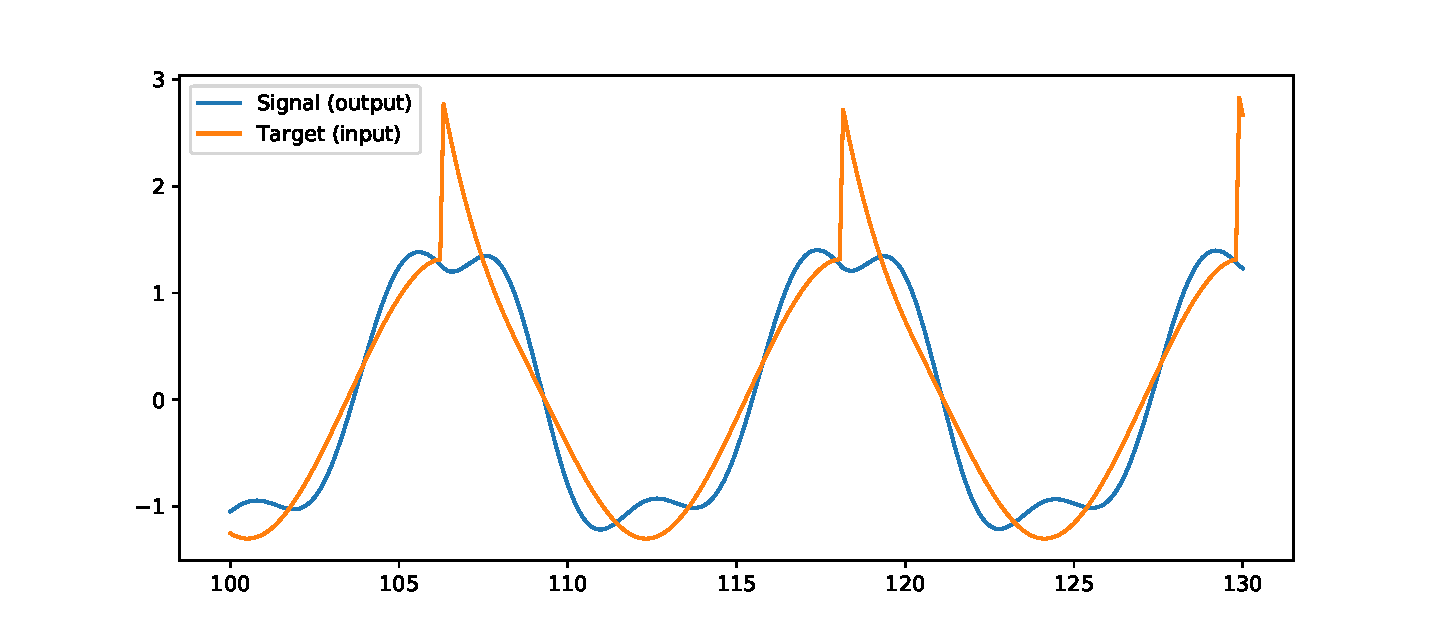
\includegraphics[width=.9\linewidth]{./perturbation.pdf}
\end{center}
\end{frame}

\begin{frame}[<+->][label={sec:org07faadf}]{Splines problems}
\begin{itemize}
\item Finite differences doesn't play nicely with splines
\item Conjecture: smooth changes in the discretisation cause non-smooth changes in the model
\begin{itemize}
\item Non-smooth map from perturbation to model somehow causes problems
\end{itemize}
\end{itemize}
\vfill
\begin{itemize}
\item Spline model somehow ceases to be valid
\begin{itemize}
\item Probable cause: data exists where knots don't, or knots exist where data don't
\item Can't understand why either would happen
\item Code errors aren't helpful
\end{itemize}
\end{itemize}
\end{frame}

\begin{frame}[<+->][label={sec:orge569ccf}]{Fixing splines}
\begin{itemize}
\item Possible solution: fiddle with finite differences step size
\begin{itemize}
\item Still doesn't work
\item Spline model error occurs within the first Newton iteration
\end{itemize}
\end{itemize}
\vfill
\begin{itemize}
\item Another idea: use evenly-spaced knots, instead of an optimized knot set
\begin{itemize}
\item Choice of exterior knots becomes difficult
\item More chance to cover entire data range with knots, to avoid invalid spline models
\item Some success
\end{itemize}
\end{itemize}
\end{frame}

\begin{frame}[label={sec:org51e44e0}]{Evenly spaced knots, small finite-differences}
\begin{center}
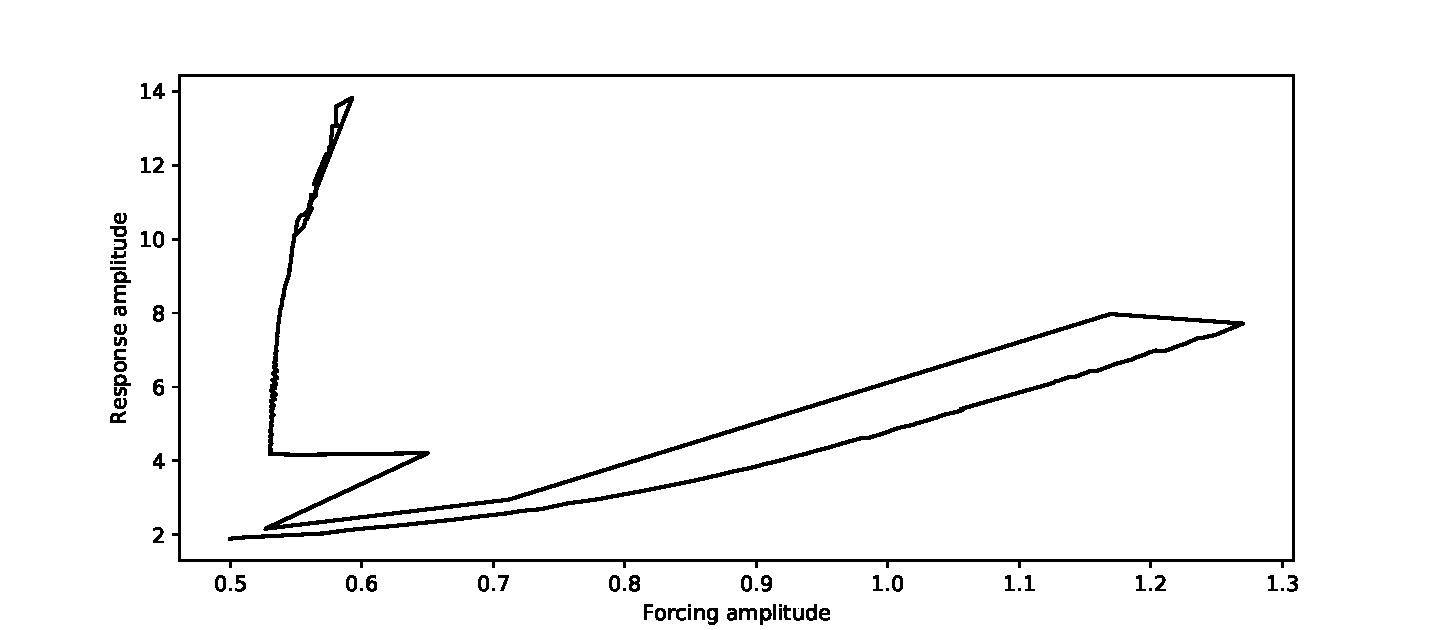
\includegraphics[width=.9\linewidth]{./spline_fail.pdf}
\end{center}

Looks bad, but no issues from invalid splines models
\end{frame}

\begin{frame}[label={sec:orgfe7fbb1}]{Evenly spaced knots, larger finite-differences}
\begin{center}
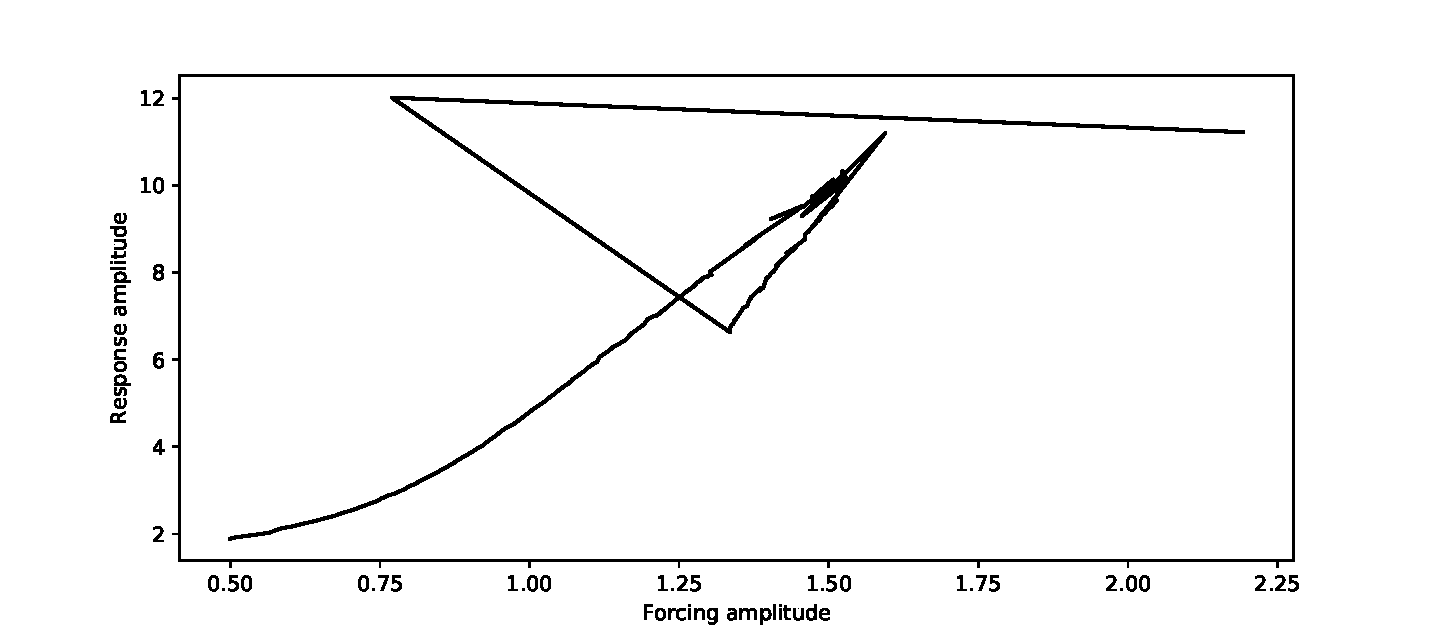
\includegraphics[width=.9\linewidth]{./spline_fail_larger_finite_differences.pdf}
\end{center}

Looks bad, but no issues from invalid splines models
\end{frame}

\begin{frame}[<+->][label={sec:org6bdcb3e}]{Hyperparameter choice}
I don't really understand what's going wrong in those plots
\vfill
\begin{itemize}
\item Played with\ldots{}
\begin{itemize}
\item Number of knots
\item Evenly spaced vs. optimized knot positions
\item Newton iteration convergence tolerance
\item Pseudo-arclength stepsize
\item Finite differences perturbation size
\end{itemize}
\end{itemize}
\vfill
\begin{itemize}
\item Never managed anything better than those plots
\end{itemize}
\vfill
\begin{itemize}
\item No understanding of why any given intervention has the effect it does
\end{itemize}
\vfill
\begin{itemize}
\item Finicky hyperparameters make the method impractical even if it did work
\end{itemize}
\end{frame}

\begin{frame}[<+->][label={sec:org6084438}]{Saving the splines approach}
\begin{itemize}
\item Try interpolating splines instead of basis splines
\begin{itemize}
\item Choose a set of points
\item Connect those points with polynomials
\item Choose polynomial coeff's for smoothness, periodicity
\end{itemize}
\end{itemize}
\vfill
\begin{itemize}
\item Discretisation becomes knot point \((x,y)\) values
\begin{itemize}
\item Or, set the \(x\) values of the knots, and let discretisation be the \(y\) values
\item Interesting aside: polynomial coeff's would also be a discretisation, but an inefficient one due to lots of redundancy; can we choose a discretisation to minimise redundant information? IO map unit eigenfunction?
\end{itemize}
\end{itemize}
\vfill
\begin{itemize}
\item Result: smooth changes in the knot points cause smooth changes in the model
\begin{itemize}
\item Should make finite differences more robust
\item Also easier to understand, more explainable: no mysterious choice of exterior knots; more intuition about how discretisation changes the model
\end{itemize}
\end{itemize}
\end{frame}

\section{Next steps}
\label{sec:orge5e60dd}
\begin{frame}[label={sec:org79c935b}]{Next steps}
\begin{itemize}
\item Try interpolating splines discretisation
\begin{itemize}
\item Start with simplest-possible (ie. non-Bayesian) approach, see what happens
\end{itemize}
\end{itemize}
\vfill
\begin{itemize}
\item Edit continuation paper
\end{itemize}
\vfill
\begin{itemize}
\item Write up extended conference paper
\end{itemize}
\vfill
\begin{itemize}
\item Choose paper and make slides for lab group meeting
\end{itemize}
\end{frame}
\end{document}
